
% LaTeX Language and campus name and format package
\documentclass[es,gi]{ifirak}\usepackage[]{graphicx}\usepackage[]{color}
%% maxwidth is the original width if it is less than linewidth
%% otherwise use linewidth (to make sure the graphics do not exceed the margin)
\makeatletter
\def\maxwidth{ %
  \ifdim\Gin@nat@width>\linewidth
    \linewidth
  \else
    \Gin@nat@width
  \fi
}
\makeatother

\definecolor{fgcolor}{rgb}{0.345, 0.345, 0.345}
\newcommand{\hlnum}[1]{\textcolor[rgb]{0.686,0.059,0.569}{#1}}%
\newcommand{\hlstr}[1]{\textcolor[rgb]{0.192,0.494,0.8}{#1}}%
\newcommand{\hlcom}[1]{\textcolor[rgb]{0.678,0.584,0.686}{\textit{#1}}}%
\newcommand{\hlopt}[1]{\textcolor[rgb]{0,0,0}{#1}}%
\newcommand{\hlstd}[1]{\textcolor[rgb]{0.345,0.345,0.345}{#1}}%
\newcommand{\hlkwa}[1]{\textcolor[rgb]{0.161,0.373,0.58}{\textbf{#1}}}%
\newcommand{\hlkwb}[1]{\textcolor[rgb]{0.69,0.353,0.396}{#1}}%
\newcommand{\hlkwc}[1]{\textcolor[rgb]{0.333,0.667,0.333}{#1}}%
\newcommand{\hlkwd}[1]{\textcolor[rgb]{0.737,0.353,0.396}{\textbf{#1}}}%
\let\hlipl\hlkwb

\usepackage{framed}
\makeatletter
\newenvironment{kframe}{%
 \def\at@end@of@kframe{}%
 \ifinner\ifhmode%
  \def\at@end@of@kframe{\end{minipage}}%
  \begin{minipage}{\columnwidth}%
 \fi\fi%
 \def\FrameCommand##1{\hskip\@totalleftmargin \hskip-\fboxsep
 \colorbox{shadecolor}{##1}\hskip-\fboxsep
     % There is no \\@totalrightmargin, so:
     \hskip-\linewidth \hskip-\@totalleftmargin \hskip\columnwidth}%
 \MakeFramed {\advance\hsize-\width
   \@totalleftmargin\z@ \linewidth\hsize
   \@setminipage}}%
 {\par\unskip\endMakeFramed%
 \at@end@of@kframe}
\makeatother

\definecolor{shadecolor}{rgb}{.97, .97, .97}
\definecolor{messagecolor}{rgb}{0, 0, 0}
\definecolor{warningcolor}{rgb}{1, 0, 1}
\definecolor{errorcolor}{rgb}{1, 0, 0}
\newenvironment{knitrout}{}{} % an empty environment to be redefined in TeX

\usepackage{alltt}

% ERABILIKO DIREN PAKETEAK %

% listings pakage is for code formating
\usepackage{listings}
% Paquete for acents and other special characters
% It is not necesary to use all this packages add or remove those you are interested on
\usepackage[utf8]{inputenc}
\usepackage{colortbl}
\usepackage[table]{xcolor}
\usepackage{graphicx}
\usepackage{wrapfig}
\usepackage{amsfonts}
\usepackage{makeidx}
\usepackage{adjustbox}
\usepackage{booktabs}
\usepackage{amsmath}

% Definition of colors
\definecolor{darkgreen}{rgb}{0,0.5,0}
\definecolor{lightgray}{rgb}{0.95,0.95,0.95}
\definecolor{gray}{rgb}{0.85,0.85,0.85}
\definecolor{white}{rgb}{1,1,1}
\definecolor{purple}{rgb}{0.51,0,0.25}
\definecolor{orange}{rgb}{0.255,0.178,0.102}
\definecolor{mygreen}{RGB}{28,172,0} 
\definecolor{mylilas}{RGB}{170,55,241}

\lstset{language=Matlab,%
    %basicstyle=\color{red},
    breaklines=true,%
    morekeywords={matlab2tikz},
    keywordstyle=\color{blue},%
    morekeywords=[2]{1}, keywordstyle=[2]{\color{black}},
    identifierstyle=\color{black},%
    stringstyle=\color{mylilas},
    commentstyle=\color{mygreen},%
    showstringspaces=false,%without this there will be a symbol in the places where there is a space
    %numbers=left,%
    %numberstyle={\tiny \color{black}},% size of the numbers
    %numbersep=20pt, % this defines how far the numbers are from the text
    emph=[1]{for,end,break},emphstyle=[1]\color{red}, %some words to emphasise
    %emph=[2]{word1,word2}, emphstyle=[2]{style},    
    backgroundcolor=\color{lightgray},
}

\DeclareMathSizes{10}{10}{10}{10}

\graphicspath{imagenes}
\renewcommand{\contentsname}{Indice}
\IfFileExists{upquote.sty}{\usepackage{upquote}}{}
\begin{document}

% Course year
\ikasturtea{2018 - 2019}
% Subject or course name
\irakasgaia{Visión por Computador}
% Title
\title{Desafío 9}
% Name of Author
\author{Mikel Dalmau}

\maketitle



%\section{Código}

\tableofcontents

\section{Enunciado}
\paragraph{}
El objetivo de esta práctica es explorar la extracción de información de profundidad de imágenes estéreo utilizando la herramienta matlab, \textit{disparity}.\\

La idea general es comprobar, para cada par de imágenes, los resultados que se obtienen variando parámetros como el Method, Blocksize, TextureThreshold y  otros. Se pueden obtener resultados cuantitativos comparando con la ground truth proporcionada en el sitio web.

\pagebreak

\section{Pruebas preliminares de los parámetros}
\paragraph{}Para hacer las pruebas he utilizado de la secuencia de imágenes \textit{Barn 2} de \cite{key-2}, las imágenes primera y sexta.\\

Cada conjunto contiene 9 imágenes (im0.ppm - im8.ppm) y dos ground-truth mapas de disparidades para las imágenes 2 y 6 (disp2.pgm and disp6.pgm). Cada ground-truth disparity tiene aplicado un factor de escala de 8. Por ejemplo, un valor de 100 en disp2.pgm significa que el pixel correspondiente en im6.ppm está 12.5 pixeles a la izquierda.\\

\subsection{Algoritmo de estimación de disparidades}
\paragraph{}La función de disparidad implementa los algoritmos básicos de BlockMatching \cite{key-3} y Semi-Global BlockMatching \cite{key-4}. En el método 'BlockMatching', la función calcula la disparidad al comparar la suma de las diferencias absolutas (SAD) de cada bloque de píxeles en la imagen. En el método de emparejamiento 'SemiGlobal', la función además fuerza una disparidad similar en bloques vecinos. Esta restricción adicional da como resultado una estimación de disparidad más completa que en el método 'BlockMatching'.\\

Los algoritmos realizan estos pasos:
\begin{enumerate}
\item Calcular una medida de contraste de la imagen utilizando el filtro Sobel.
\item Calcular la disparidad para cada píxel en I1. 
\item Marcar los elementos del mapa de disparidad, disparityMap, que no se calcularon de manera confiable. La función utiliza –realmax ('single') para marcar estos elementos.\\
\end{enumerate}

La siguiente imágen muestra las diferencias de resultados entre un algoritmo y el otro.\\

\begin{tabular}{c|c}
    \toprule
    	\bfseries Block Matching &
    	\bfseries SemiGlobal \\
    \midrule
    	\adjustimage{height=6cm,valign=m}{imagenes/barn_1-6-dr-0-32_dm}
		& \adjustimage{height=6cm,valign=m}{imagenes/barn_1-6-dr-0-32}\\
    \bottomrule
\end{tabular}

\subsection{Disparity Range}
\paragraph{} El rango de disparidad depende de la distancia entre las dos cámaras y la distancia entre las cámaras y el objeto de interés. Aumenta cuando las cámaras estén alejadas o los objetos están cerca de las cámaras.\\

Para determinar una disparidad razonable para la configuración puede utilizarse el anaglifo estéreo de las imágenes de y la herramienta para medir distancias entre pares de puntos correspondientes.\\

\begin{figure}[hbtp]
\centering
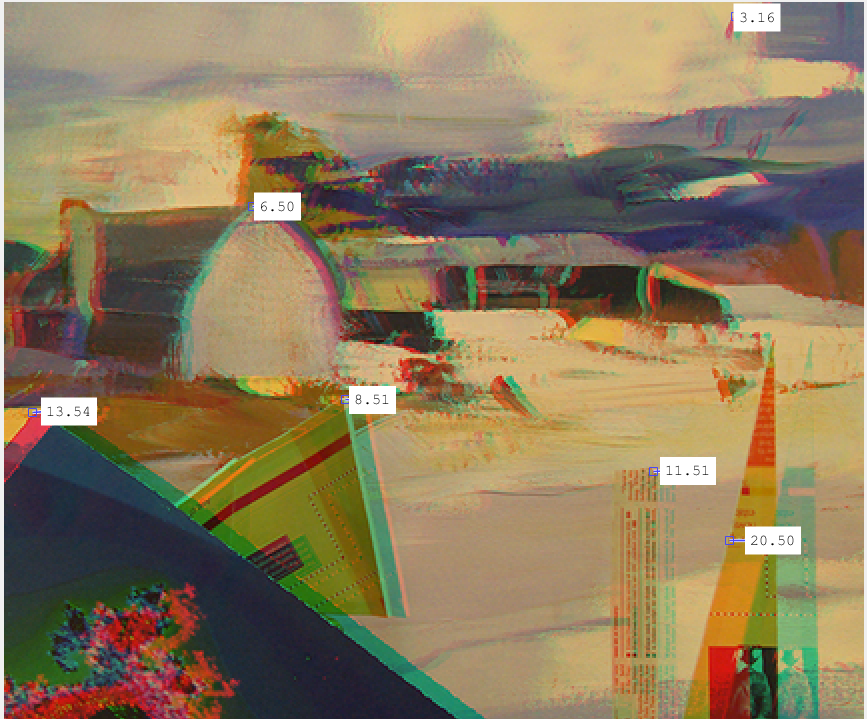
\includegraphics[scale=0.5]{imagenes/barn_1-6-dr-Distances.png}
\caption{Medidas de disparidad a distintas profundidades entre las imágenes 1 y 6.}
\end{figure}

\paragraph{} La diferencia entre MaxDisparity y MinDisparity debe ser divisible por 16 y por las medidas tomadas, las disparidades entre las anteriores imágenes varían entre 6 y 25 más o menos. Si la cámara utilizada para tomar I1 estaba a la derecha de la cámara utilizada para tomar I2, entonces MinDisparity debe ser negativo.\\

Las siguiente tabla muestra el mapa de disparidades calculado utilizando distintos rangos, podemos distinguir cómo los colores están corridos hacia el rojo cuando hemos elegido unos márgenes muy bajos o cómo están corridos al azul si los márgenes son muy altos. Idealmente, si el rango es el apropiado, habrá mayor contraste entre los objetos a distintas profundidades, me ha parecido que el rango [0, 32] es razonable para estas imágenes.\\

\begin{tabular}{p{2cm}c|p{2cm}c}
    \toprule
    	disparity = [-32, 32]
		& \adjustimage{height=4cm,valign=m}{imagenes/barn_1-6-dr-32-32}
		& disparity = [0, 32]
		& \adjustimage{height=4cm,valign=m}{imagenes/barn_1-6-dr-0-32}\\
		
	\midrule
		disparity = [4, 20]
		& \adjustimage{height=4cm,valign=m}{imagenes/barn_1-6-dr-4-20}
		& disparity = [0, 64]
		& \adjustimage{height=4cm,valign=m}{imagenes/barn_1-6-dr-0-64}\\
    \bottomrule
\end{tabular}

\pagebreak
\subsection{Block Size}
\paragraph{} El block size tiene que ser un entero impar en el rango [5,255]. Este valor establece el ancho para el tamaño de bloque cuadrado. La función utiliza el bloque cuadrado de píxeles para las comparaciones entre I1 e I2.\\

La siguiente tabla muestra los efectos de variar el tamaño de bloque y en estos casos cuanto mayor el tamaño de bloque más precision se pierde a la hora de comparar la suma de las diferencias absolutas, llegando incluso a distorsionar el resultado cuando el tamaño de bloque es muy grande. Para el uso actual y el tamaño de imágen actual el mínimo tamaño de bloque es el más apropiado, solo interesaría aumentarlo para mejorar el rendimiento del algoritmo en imágenes grandes y cuando la precisión sea menos importante que la velocidad de cómputo.\\

En las siguientes imágenes se ha utilizado el disparity range [0, 32].\\	

\begin{tabular}{p{2cm}c|p{2cm}c}
    \toprule
    	BlockSize = 5
		& \adjustimage{height=4.5cm,valign=m}{imagenes/barn_1-6-dr-0-32-bs-5}
		& BlockSize = 7
		& \adjustimage{height=4.5cm,valign=m}{imagenes/barn_1-6-dr-0-32-bs-7}\\
		
	\midrule
		BlockSize = 13
		& \adjustimage{height=4.5cm,valign=m}{imagenes/barn_1-6-dr-0-32-bs-13}
		& BlockSize = 55
		& \adjustimage{height=4.5cm,valign=m}{imagenes/barn_1-6-dr-0-32-bs-55}\\
		
	\midrule
		BlockSize = 105
		& \adjustimage{height=4.5cm,valign=m}{imagenes/barn_1-6-dr-0-32-bs-105}
		& BlockSize = 255
		& \adjustimage{height=4.5cm,valign=m}{imagenes/barn_1-6-dr-0-32-bs-255}\\
    \bottomrule
\end{tabular}

\pagebreak
\subsection{Contrast Threshold}

\paragraph{}El umbral de contraste es un valor escalar en el rango (0,1] y define un rango aceptable de valores de contraste, cuanto mayor este parámetro, menos pixels serán marcados como no confiables. Por defecto tiene el valor 0.5.\\
 
Cambiar este parámetro en esta imágen en particular no produce muchas diferencias pues la mayoría de pixels se están marcando como confiables. Aún así pueden verse varios píxels en algunas zonas que ahora se han marcado como confiables.\\

\begin{tabular}{p{2cm}c|p{2cm}c}
    \toprule
    	ContrastThreshold = 0.01
		& \adjustimage{height=4.5cm,valign=m}{imagenes/barn_1-6-ct-001}
		& ContrastThreshold = 0.25
		& \adjustimage{height=4.5cm,valign=m}{imagenes/barn_1-6-ct-025}\\
		
	\midrule
		ContrastThreshold = 0.75
		& \adjustimage{height=4.5cm,valign=m}{imagenes/barn_1-6-ct-075}
		& ContrastThreshold = 1
		& \adjustimage{height=4.5cm,valign=m}{imagenes/barn_1-6-ct-1}\\
		
    \bottomrule
\end{tabular}
 
 \pagebreak
\section{Resultados}
\paragraph{} La siguiente tabla muestra las disparidades entre la imágen 0 y el resto. 
Los paramétros utilizados en todas las pruebas para calcular las disparidades son (SemiGlobal, disparity range [0 32], Block Size - 5, Contras Threshold 0.5).\\
 
\begin{tabular}{ccc}
    \toprule
    	\adjustimage{height=5cm,valign=m}{imagenes/barn_0_1}
		& \adjustimage{height= 5cm,valign=m}{imagenes/barn_0_2}
		& \adjustimage{height= 5cm,valign=m}{imagenes/barn_0_3}\\
		
		 \adjustimage{height=5cm,valign=m}{imagenes/barn_0_4}
		& \adjustimage{height= 5cm,valign=m}{imagenes/barn_0_5}
		& \adjustimage{height=5cm,valign=m}{imagenes/barn_0_6}\\
		
		\adjustimage{height=5cm,valign=m}{imagenes/barn_0_7}
		& \adjustimage{height=5cm,valign=m}{imagenes/barn_0_8}
		&\\
				
    \bottomrule
\end{tabular}

\paragraph{} La siguiente tabla muestra, para cada serie de imágenes, la primera, el ground truth con respecto a la sexta y el disparity map calculado utilizando los parámetros descritos anteriormente.\\

\begin{tabular}{p{1.5cm}ccc}
    \toprule
    	\bfseries Name &
    	\bfseries Left Image &
    	\bfseries Ground Truth &
    	\bfseries Disparity Map \\
    \midrule
   barn1 &	\adjustimage{height=4cm,valign=m}{imagenes/barn1_L}
		& \adjustimage{height=4cm,valign=m}{imagenes/barn1_gt}
		& \adjustimage{height=4cm,valign=m}{imagenes/barn1_dm}\\

	&&&\\
		
	barn2&	\adjustimage{height=4cm,valign=m}{imagenes/barn2_L}
		& \adjustimage{height= 4cm,valign=m}{imagenes/barn2_gt}
		& \adjustimage{height= 4cm,valign=m}{imagenes/barn2_dm}\\
		
	&&&\\

	bull &	\adjustimage{height=4cm,valign=m}{imagenes/bull_L}
		& \adjustimage{height=4cm,valign=m}{imagenes/bull_gt}
		& \adjustimage{height= 4cm,valign=m}{imagenes/bull_dm}\\
	
	&&&\\

	venus &	\adjustimage{height=4cm,valign=m}{imagenes/venus_L}
		& \adjustimage{height= 4cm,valign=m}{imagenes/venus_gt}
		& \adjustimage{height= 4cm,valign=m}{imagenes/venus_dm}\\
				
    \bottomrule
\end{tabular}

	\begin{tabular}{p{1.5cm}ccc}
    \toprule
    	\bfseries Name &
    	\bfseries Left Image &
    	\bfseries Ground Truth &
    	\bfseries Disparity Map \\
    \midrule

	saw &	\adjustimage{height=4cm,valign=m}{imagenes/saw_L}
		& \adjustimage{height= 4cm,valign=m}{imagenes/saw_gt}
		& \adjustimage{height= 4cm,valign=m}{imagenes/saw_dm}\\

	&&&\\

	poster&	\adjustimage{height=4cm,valign=m}{imagenes/poster_L}
		& \adjustimage{height=4cm,valign=m}{imagenes/poster_gt}
		& \adjustimage{height= 4cm,valign=m}{imagenes/poster_dm}\\
				
    \bottomrule
\end{tabular}

\pagebreak
\subsection{Cálculo del error}
\paragraph{} Para calcular el error he seguido el método descrito en \cite{ket-4}, tratando como errores todas las disparidades con una diferencia mayor que 1 respecto al ground truth y descartando los pixels a 0 (en vez de interpolar sus valores a con sus vecinos).\\

De los resultados podemos extraer que a mayor cantidad e bordes y ángulos cerrados los errores aumentan, ya que en las superficies planas interiores los algoritmos resultan más eficaces.\\

\begin{table}[hbtp]
\centering
\begin{tabular}{ccccccc}
\toprule
\bfseries Imagen & barn1 &  barn2 &     bull & venus &  poster &  sawtooth\\
\midrule
\bfseries \% errores &  7.3 &    7.4 &   1.6  &   2.8 &    2.7 &    7.3 \\
\bottomrule
\end{tabular}
\end{table}

\begin{figure}[hbtp]
\centering
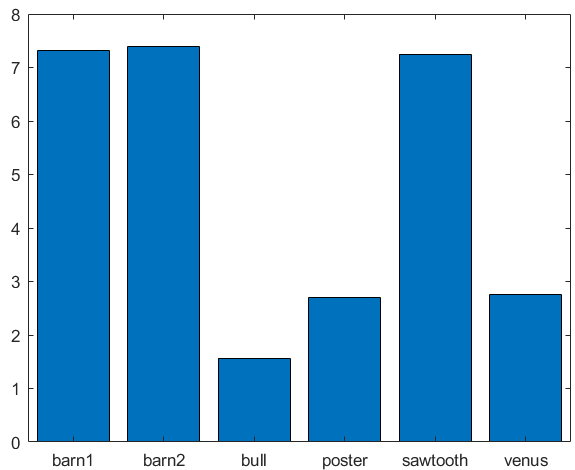
\includegraphics[scale=0.6]{imagenes/results.png}
\caption{Porcentaje de errores.}
\end{figure}

\begin{thebibliography}{arauak}
	
	\bibitem[MatLab 1]{key-1} Matlab documentación oficial:\textit{https://www.mathworks.com/help/vision/ref/disparity.html}
	
	\bibitem[Middlebury, 2001]{key-2} Stereo Images, \textit{http://vision.middlebury.edu/stereo/data/}
	
	\bibitem[Konolige, 1997]{key-3} Konolige, K., \textit{Small Vision Systems: Hardware and Implementation, Proceedings of the 8th International Symposium in Robotic Research}, pages 203-212, 1997.

\bibitem[Hirschmuller, 2004]{key-4} Hirschmuller, H., Accurate and Efficient Stereo Processing by Semi-Global Matching and Mutual Information, International Conference on Computer Vision and Pattern Recognition, 2005.

\end{thebibliography}



\end{document}
